%%%%%%%%%%%%
%
% $Autor: Wings $
% $Datum: 2019-03-05 08:03:15Z $
% $Pfad: NAgicWand,tex $
% $Version: 4250 $
% !TeX spellcheck = en_GB/de_DE
% !TeX encoding = utf8
% !TeX root = filename 
% !TeX TXS-program:bibliography = txs:///biber
%
%%%%%%%%%%%%


\chapter{Magic Wand}


\begin{itemize}
  \item Als Mikrocontrollerboard wird ein Arduino Nano 33 BLE verwendet:
    
          \URL{https://docs.arduino.cc/hardware/nano-33-ble/}
  \item Betrieben wird das Controllerboard mit einer Lithium Batterie CR2032: \cite{Energizer:2018}
  
        \URL{https://data.energizer.com/pdfs/cr2032.pdf}           
        
  \item Der Stab ist aus Acryl: 
  
        \URL{https://acrylhaus.com/Rundstab-aus-Acrylglas-XT-mit-Luftblasen}
  \item Für den 3D-Druck wurde PETG Filament verwendet:
  
      \URL{https://www.material4print.de/filament/petg/31/petg-tiefschwarz?c=15}
            
\end{itemize}


\section{Attention}

An drei Ausgangpins des Controllerboards ist, über Vorwiderstände von 180 Ohm, eine RGB-LED
angeschlossen.

Der Zauberstab lässt sich über die eingebaute Micro-USB Schnittstelle programmieren.

Dazu muss der Zauberstab geöffnet und der Jumper im inneren geschlossen (gesteckt werden).


\textbf{ACHTUNG vor dem Stecken des Jumpers muss der Stab ausgeschaltet sein und er darf
nicht eingeschaltet werden, solange der Jumper steckt!!}


\section{Gehäuse}


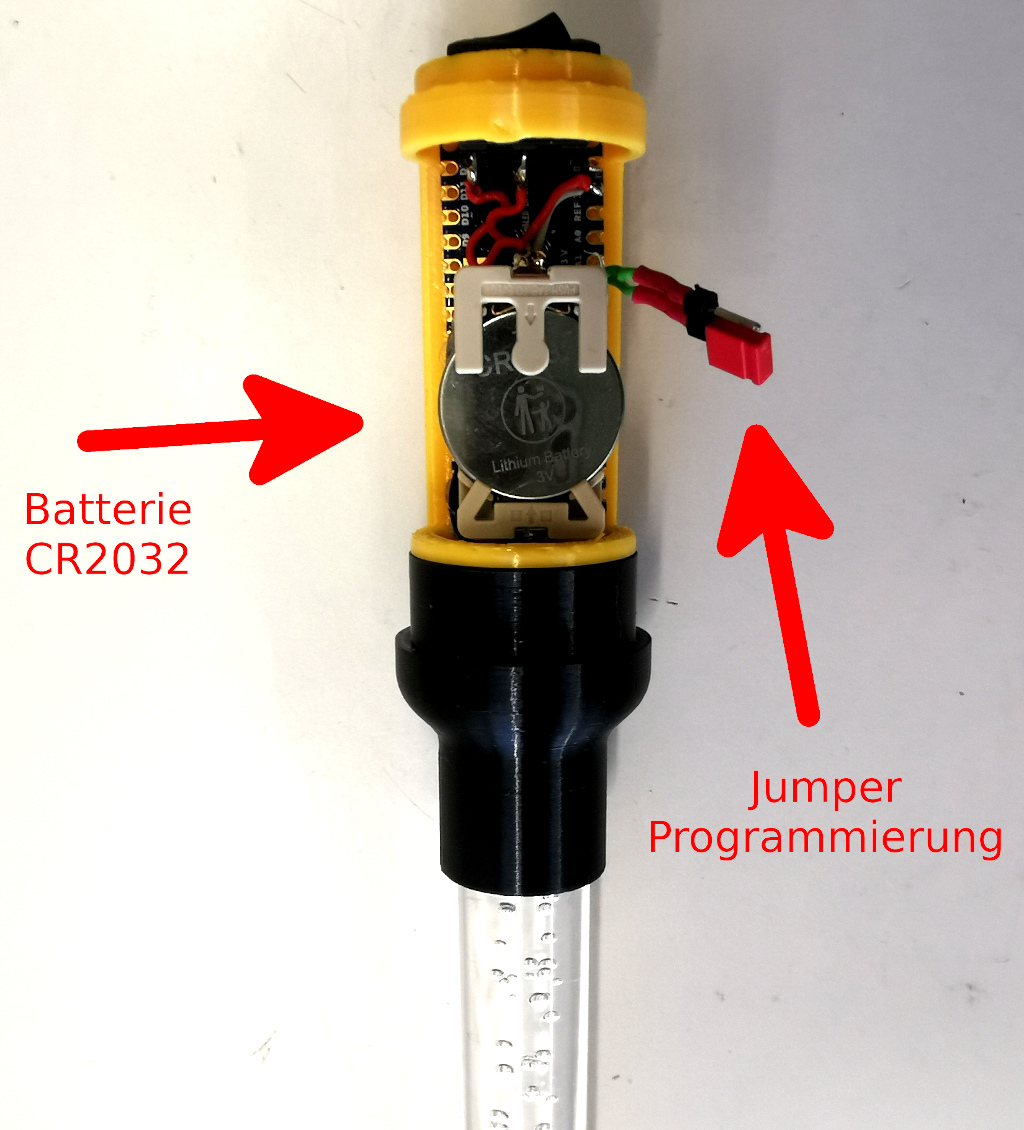
\includegraphics[width=0.8\textwidth]{MagicWand/MagicWandS}

\bigskip

Die Gehäusekonstruktion wurde mit Fusion 360 erstellt.

\bigskip

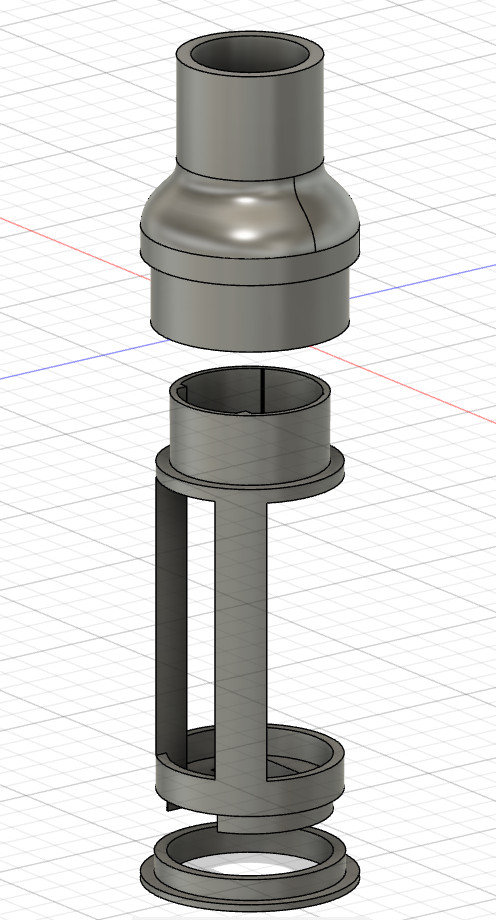
\includegraphics[width=0.3\textwidth]{MagicWand/MagicWandCAD01}
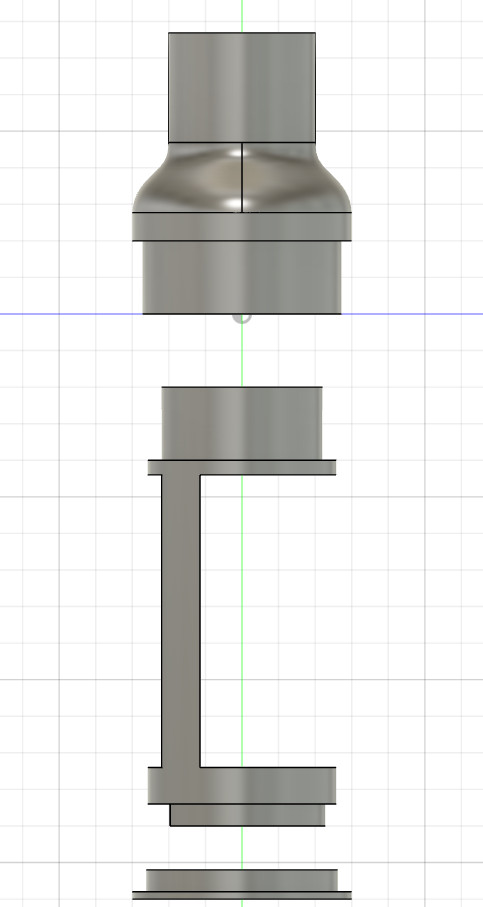
\includegraphics[width=0.3\textwidth]{MagicWand/MagicWandCAD02}
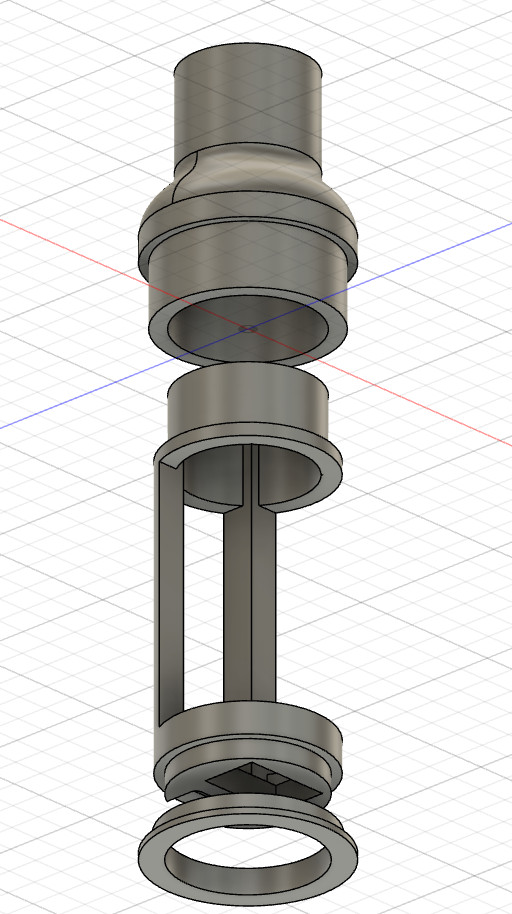
\includegraphics[width=0.3\textwidth]{MagicWand/MagicWandCAD03}

\bigskip

{
  \captionof{code}{Einschalten der Farben der RGB-Led}
  \ArduinoExternalO{../../Code/Nano33BLESense/MagicWand/MagicWandOnOff.ino}
}


{
  \captionof{code}{Farbwechsel der RGB-Led}
  \ArduinoExternalO{../../Code/Nano33BLESense/MagicWand/MagicWandPWM.ino}
}